\documentclass[pdftex,12pt,a4paper]{article}

\usepackage{graphicx}  
\usepackage[margin=2.5cm]{geometry}
\usepackage{breakcites}
\usepackage{indentfirst}
\usepackage{pgfgantt}
\usepackage{pdflscape}
\usepackage{float}
\usepackage{epsfig}
\usepackage{epstopdf}
\usepackage[cmex10]{amsmath}
\usepackage{stfloats}
\usepackage{multirow}

\renewcommand{\refname}{REFERENCES}
\linespread{1.3}

% REQUIRED FOR INSETYING SOME SHITASS ASSEMBLY CODE INTO TO LATEX BIATCH fuck this retarded thing, science my ass
\usepackage{listings}
\usepackage{xcolor}
\definecolor{codegreen}{rgb}{0,0.6,0}
\definecolor{codegray}{rgb}{0.5,0.5,0.5}
\definecolor{codepurple}{rgb}{0.58,0,0.82}
\definecolor{backcolthe}{rgb}{0.95,0.95,0.92}
\definecolor{CommentGreen}{rgb}{0,.6,0}
% bu salak seyin son satiri bosluk olunca calismiyor kendimi sikcem simdi
% Icine comment de konmuyor

\lstset{
    numbers=left,
    basicstyle=\small\ttfamily,
    numberstyle=\tiny,
    keywordstyle=\color{blue}\bfseries,
    keywordsprefix=B,
    language={[x86masm]Assembler},
    breaklines=true,
    commentstyle=\color{codegreen},
    keywordstyle=\color{blue},
    keywordstyle=[2]\color{orange},
    keywordstyle=[3]\color{codegray},
    numberstyle=\tiny\color{codegray},
    stringstyle=\color{codepurple},
    showtabs=false,
    frame=single,
    keepspaces,
}



\usepackage{mathtools}
%\newcommand{\HRule}{\rule{\linewidth}{0.5mm}}
\thispagestyle{empty}
\begin{document}
\begin{titlepage}
\begin{center}
\textbf{}\\
\textbf{\Large{ISTANBUL TECHNICAL UNIVERSITY}}\\
\vspace{0.5cm}
\textbf{\Large{COMPUTER ENGINEERING DEPARTMENT}}\\
\vspace{2cm}
\textbf{\Large{BLG 351E\\ MICROCOMPUTER LABORATORY\\ EXPERIMENT REPORT}}\\
\vspace{2.8cm}
\begin{table}[ht]
\centering
\Large{
\begin{tabular}{lcl}
\textbf{EXPERIMENT NO}  & : & 4 \\
\textbf{EXPERIMENT DATE}  & : & 23.10.2019 \\
\textbf{LAB SESSION}  & : & WEDNESDAY - 13.30 \\
\textbf{GROUP NO}  & : & G10 \\
\end{tabular}}
\end{table}
\vspace{1cm}
\textbf{\Large{GROUP MEMBERS:}}\\
\begin{table}[ht]
\centering
\Large{
\begin{tabular}{rcl}
150170062  & : & Mehmet Fatih YILDIRIM \\
150180704  & : & Cihat AKK\.{I}RAZ \\
150180705  & : & Batuhan Faik DER\.{I}NBAY \\
150180707  & : & Fatih ALTINPINAR \\
\end{tabular}}
\end{table}
\vspace{2.8cm}
\textbf{\Large{FALL 2019-2020}}

\end{center}

\end{titlepage}

\newpage


\thispagestyle{empty}
\addtocontents{toc}{\contentsline {section}{\numberline {}FRONT COVER}{}}
\addtocontents{toc}{\contentsline {section}{\numberline {}CONTENTS}{}}
\setcounter{tocdepth}{4}
\tableofcontents
\clearpage

\setcounter{page}{1}


\section{INTRODUCTION}

Subroutines are very important in assembly language. Using them program size decreases and codes are getting more understandable. While using subroutines, some parameters should be enter this subroutine and return value end of the some calculation. End of the subroutine, program should be continue its execution with the instruction after subroutine call in the main program. Entering parameters to the subroutine, return values and PC address of instruction after the subroutine call should be stored somewhere. 
\newline{}
Stack is a special memory about to use during execution of the program. Coding in assembly language with MSP430G2553 microprocessor, PUSH and POP commands are using to add value to the top of the stack and remove value from top of the stack with copying it a register. So, stack is a LAST IN FIRST OUT(LIFO) structure.
While calling a subroutine with CALL instruction, address value of next instruction after subroutine call in the subroutine is pushed to the stack. Thus, the program can continue to run after the subroutine operations.

\section{MATERIALS AND METHODS}

This experiment is conducted via using MSP430G2553 microprocessor. This microprocessor is programmed using Code Composer Studio according to desired tasks on the experiment handout. During coding below sources are used:

\begin{itemize}
    \item MSP430 Education Board Manual \cite{ref2}
    \item MSP430 Architecture Chapter 4 \cite{ref3}
    \item MSP430 Instruction Set \cite{ref4}
    \item Supplementary Chapter 6 General Purpose IO \cite{ref5}
\end{itemize}

\subsection{Part 1}

\newline{}
In the first part of the experiment, a new CCS Project is created as choosing "MSP430G2553" as the target and "Empty Assembly Project" as the project template. Then, the codes in the experiment booklet(also see Figure \ref{code:part1}) are run and debugged. While debugging, values in the registers and stack are examined and table(see Figure \ref{fig:part1} is filled with these values.


\begin{figure}[H]
    \centering
    \begin{lstlisting}[language={[x86masm]Assembler}]
Setup   mov #array, r5
        mov #resultArray, r10
            
Mainloop mov.b   @r5,r6
            inc r5
            call #func1
            mov.b r6, 0(r10)
            cmp #lastElement, r5
            jlo Mainloop
            jmp finish

func1   xor.b #0FFh, r6
        mov.b r6, r7
        call #func2
        mov.b r7,r6
        ret
            
func2   inc.b r7
        ret
            
;Integer array
array   .byte 127, -128,0,55
lastElement
        nop
    \end{lstlisting}
    \label{code:part1}
    \caption{Assembly Code of Part 1}
\end{figure}

For better understanding, further examination of the code, line by line if necessary, is required:

\begin{itemize}
    \item Line 1-2: Address of array is moved to R5 and address of resultArray is move to R10.

    \item Line 4:  The value in pointed by R5 is moved to R6. (Indirect Addressing)

    \item Line 5: The value of R5 is increased by 1.

    \item Line 6: func1 is called. Address of the next instruction(PC+2) in line 7 is pushed to stack to return main function after finishing operation in function. Address of SP is changed because of adding new value to stack. PC value will be changed to execute func1 with this instruction.
    
    \item Line 12: R6 value is changed with X0R operation.

    \item Line 13: R6 value is moved to R7.
    
    \item Line 14: func2 is called. Address of the next instruction(PC+2) in line 15 is pushed to stack to return func1 function after finishing operation in func2. Address of SP is changed because of adding new value to stack. PC value will be changed to execute func2 with this instruction.
    
    \item Line 18: R7 value is increased by 1.

    \item Line 19: With RET instruction function is returning address(Line 15) that is pushed to stack in line 14. This value is popped from stack and appointed as new PC.
    
    \item Line 15: R7 value is moved to R6.
    
    \item Line 16: With RET instruction function is returning address(Line 7) that is pushed to stack in line 6. This value is popped from stack and appointed as new PC.
    
    \item Line 7: R6 value is moved to R10.
    
    \item Line 8: Address of last element of array is compared with R5 to see if it's at the end of the list.

    \item Line 9: Jump Mainloop again if value in R5 is lower than address of last element of array.
    
    \item Line 10: If R5 is bigger than lastElement or equal to lastElement finish program.
\end{itemize}{}

\begin{figure}[H]
    \centering
    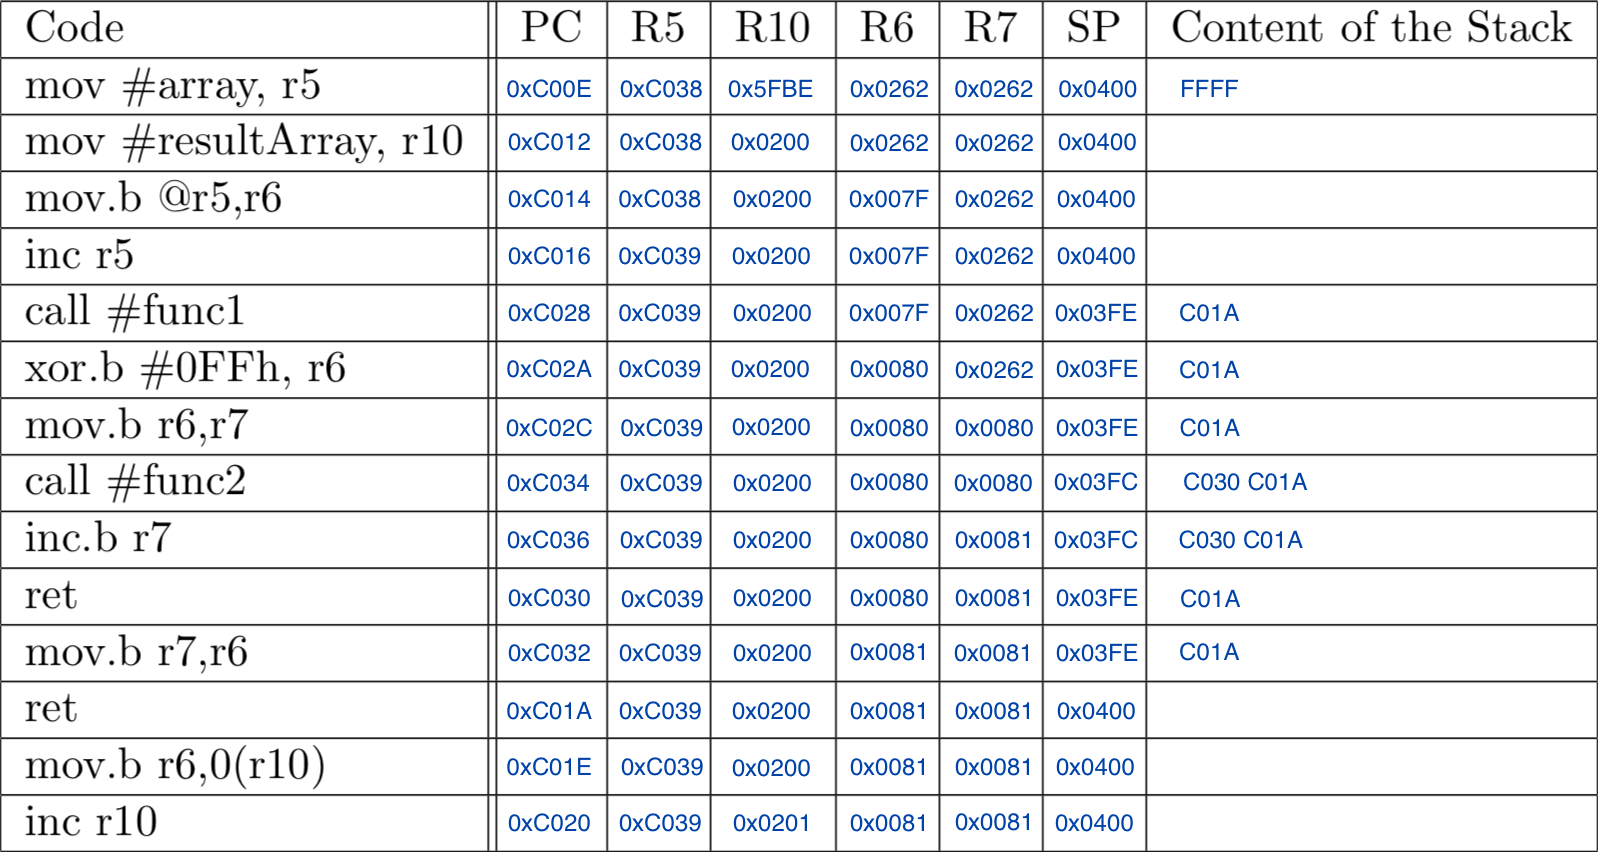
\includegraphics[width=1\textwidth]{table.png}
    \caption{Registers and stack status while Debugging}
    \label{fig:part1}
\end{figure}


\subsection{Part 2}
\newline
In this section the team was asked to write four functions, namely addition, subtraction, multiplication and division, in assembly language.

In order to implement the given task, team created following pieces of codes given in Figures \ref{fig:addFunction}.1 - \ref{fig:divFunction}.4.

Under each figure, explanation of the code can be found.

\begin{figure}[H]
    \centering
\begin{lstlisting}[language={[x86masm]Assembler}, numbers=left]
Add_func	push	r4
		push	r5
		mov		6(sp), r4
		mov		8(sp), r5
		add		r5, r4
		mov		r4, 10(sp)
		pop		r5
		pop		r4
		ret
    \end{lstlisting}
    \label{fig:addFunction}
    \caption{Addition Function}
\end{figure}

\begin{itemize}
    \item Line 1-2: Pushes registers to be used to stack in order to keep their value.
    \item Line 3-4: Retrieves caller parameters from stack
    \item Line 5-6: Does the addition and pushes to result location of the stack
    \item Line 7-8: Loads used registers with previous values for later use in caller function
    \item Line 9: Returns back to next instruction after the caller function

\end{itemize}

\begin{figure}[H]
    \centering
\begin{lstlisting}[language={[x86masm]Assembler}, numbers=left]
Sub_func	push	r4
		push	r5
		mov		6(sp), r4
		mov		8(sp), r5
		sub		r5, r4
		mov		r4, 10(sp)
		pop		r5
		pop		r4
		ret
    \end{lstlisting}
    \label{fig:subFunction}
    \caption{Subtraction Function}
\end{figure}

\begin{itemize}
    \item Line 1-2: Pushes registers to be used to stack in order to keep their value.
    \item Line 3-4: Retrieves caller parameters from stack
    \item Line 5-6: Does the subtraction and pushes to result location of the stack
    \item Line 7-8: Loads used registers with previous values for later use in caller function
    \item Line 9: Returns back to next instruction after the caller function

\end{itemize}

\begin{figure}[H]
    \centering
\begin{lstlisting}[language={[x86masm]Assembler}, numbers=left]
; R6 = i
Mul_func	push	r4
		push	r5
		push	r6
		mov		#0, r6
		mov		8(sp), r4
		mov		10(sp), r5
for_mul		cmp		r5, #0
		jz		mul_return
		add		r4, r6
		dec		r5
		jmp		for_mul
mul_return	mov		r6, 12(sp)
		pop		r6
		pop		r5
		pop		r4
		ret
    \end{lstlisting}
    \label{fig:mulFunction}
    \caption{Multiplication Function}
\end{figure}

\begin{itemize}
    \item Line 2-4: Pushes registers to be used to stack in order to keep their value.
    \item Line 5-7: Retrieves caller parameters from stack and initializes temporary registers, namely R6 in this case 
    \item Line 8-12: Does the multiplication until calling parameter "b" is 0. Decrements "b" every step so it is utilized as an index. The parameter "a" is added to itself "b" times and stored in R6 in the loop.
    \item Line 13-16: Stores the return value R6 and loads used registers with previous values for later use in caller function
    \item Line 17: Returns back to next instruction after the caller function

\end{itemize}

\begin{figure}[H]
    \centering
\begin{lstlisting}[language={[x86masm]Assembler}, numbers=left]
Div_func	push	r4
		push	r5
		push	r6
		mov		#0, r6
		mov		8(sp), r4
		mov		10(sp), r5
for_div		cmp		r5, r4
		jl		div_return
		sub		r5, r4
		inc		r6
		jmp		for_div
div_return	mov		r6, 12(sp)
		pop		r6
		pop		r5
		pop		r4
		ret
    \end{lstlisting}
    \label{fig:divFunction}
    \caption{Division Function}
\end{figure}

\begin{itemize}
    \item Line 1-3: Pushes registers to be used to stack in order to keep their value.
    \item Line 4-6: Retrieves caller parameters from stack and initializes temporary registers, namely R6 in this case. 
    \item Line 7-11: Does the division until calling parameter "a" is less than "b". Subtracts "b" from "a" every step and increments R6 every step so R6 is utilized as the result. The parameter "b" is subtracted from "a" R6 times in the loop so R6 holds the integer division value.
    \item Line 12-15: Stores the return value R6 and loads used registers with previous values for later use in caller function
    \item Line 16: Returns back to next instruction after the caller function

\end{itemize}

\newpage
\subsection{Part 3}
In this part of the experiment call of a subroutine from another subroutine needed to be implemented. Since add subroutine from part 2 has to be used in this part, both functions should use stack as intended for not overriding each other's data thus producing a wrong result. 

\newline{}
In order to obtain a subroutine that calculates permutation the team decided on the following piece of code given in Figure \ref{code:permFunc}.

\begin{figure}[H]
    \centering
\begin{lstlisting}[language={[x86masm]Assembler}, numbers=left]
Perm_func	push	r4
		push	r5
		push	r6
		mov		#1, r6
		mov		8(sp), r4
		mov		10(sp), r5
for_perm	cmp		#0, r5
		jz		perm_return
		push	r6
		push	r6
		push	r4
		call	Mul_func
		pop		r4
		pop		r6
		pop		r6
		dec		r4
		dec		r5
		jmp		for_perm
perm_return	mov		r6, 12(sp)
		pop		r6
    	pop		r5
		pop		r4
		ret
\end{lstlisting}
    \caption{Permutation Function}
    \label{code:permFunc}
\end{figure}

\begin{itemize}
    \item Line 1-3: Pushing registers that is going to be used during execution of the subroutine so they don't lose their value. So functionality of the caller function or main routine won't be disrupted.
    \item Line 4: $R6$ will hold the end result. It is also the register that one of the numbers that will be multiplied.
    \item Line 5-6: Loading function parameters relative to the stack pointer. 
    \item Line 7-8: When $P(n, r)$ (n = R4, r = R5) needs to be calculated, the result can be obtained by multiplying all the of the numbers starting from $n$ to $n - r + 1$. In this multiplication there will be $r$ many numbers, thus implementation of a for loop is required which will work $r$ times.
    \item Line 9-15: Multiplication function is called with the parameters $R6$ which is the current result of the multiplication and $R4$ which is a number from $n(n-1)...(n-r+1)$. Result is loaded to R6.
    \item Line 16-17: Decrementing $R4$ in order to obtain next value from $n(n-1)...(n-r+1)$ that needs to be multiplied and $R5$ so for loop is called $r$ many times.
    \item Line 18: Jump to for loop
    \item Line 19: Writing the result to the stack relative to the stack pointer by 12 bytes. Since there are 3 registers that are pushed to be saved, a return address, 2 function parameters which is in total $(3 + 1 + 2) x 2 = 12$.
    \item Line 20-22: Loading original values of the registers
    \item Line 23: Returning to the address where this function called in the first place.
\end{itemize}

\newline{}
In order to obtain a recursive function that calculates factorial the team decided on the following piece of code given in Figure \ref{code:factFunc}.

\begin{figure}[H]
    \centering
\begin{lstlisting}[language={[x86masm]Assembler}, numbers=left]
Fact_func	push	r4
		push	r5
                mov		6(sp), r4
		cmp		#2, r4
		jl		fact_rtrn
		mov		r4, r5
		dec		r5
		push	r5
		push	r5
		call	Fact_func
		pop		r5
		pop		r5
		push	r4
		push	r5
		push	r4
		call	Mul_func
		pop		r4
		pop		r4
		pop		r4
		mov		r4, 4(sp)
		pop		r5
		pop		r4
		ret
fact_rtrn       mov		#1, 4(sp)
		pop		r5
		pop		r4
		ret
\end{lstlisting}
    \caption{Factorial Function}
    \label{code:factFunc}
\end{figure}

\begin{itemize}
    \item Line 1-2: Saving the values of register that will used during this operation
    \item Line 3: Loading the parameter of the function from stack.
    \item Line 4-5 and Line 24-27: Exit condition of the recursive function. When $n<2$, $fact(n)$ will return 1 since $fact(1)=fact(0)=1$
    \item Line 6-7: Since $n-1$ is required to calculate $fact(n-1)$ value of $R4$ is copied to $R5$ then decremented.
    \item Line 8-12: Called $fact(n-1)$ and result will be written on the $R5$ which was holding the value of $n-1$ now holds result of the $fact(n-1)$
    \item Line 13-19: A function call is made in order to obtain the value of $fact(n)$ which is equal to $n x (n-1)$ the value of $n$ was stored in $R4$ and result of $fact(n-1)$ is stored in $R5$ thus these registers are pushed to stack.
    \item Line 20: Result of the $fact(n)$ is written to stack.
    \item Line 21-23: Popping original values of the used registers then returning.
\end{itemize}

\subsection{Part 4}
We could use 16 bits in a way that they would represent some necessary information about the number, for example; its sign, etc. This way, we could represent fractional part of a number as well as its integer part. Some format like IEEE 754 half-precision binary floating-point format (binary16) can be used in this manner. According to Wikipedia, "The IEEE 754 standard specifies a binary16 as having the following format:

    Sign bit: 1 bit
    Exponent width: 5 bits
    Significand precision: 11 bits (10 explicitly stored)

The format is laid out as follows:

\begin{figure}[H]
    \centering
    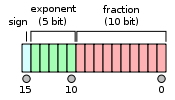
\includegraphics[width=0.3\textwidth]{IEEE_binary16.png}
    \caption{binary16 format}
    \label{}
\end{figure}

The format is assumed to have an implicit lead bit with value 1 unless the exponent field is stored with all zeros. Thus only 10 bits of the significand appear in the memory format but the total precision is 11 bits. In IEEE 754 parlance, there are 10 bits of significand, but there are 11 bits of significand precision ${(log10(211) ≈ {\approx} 3.311}$ decimal digits, or 4 digits ${\pm}$ slightly less than 5 units in the last place). ..."\cite{wiki}

\newpage

\section{RESULTS}%conc kısmı niye benim cümlelerim sen kimsin 
In the first part of the experiment, the team had try to understand to the given code as using debug mode and observing register and stack values step by step. The team observed what happens on the stack and on the some special registers while calling CALL, RET, JMP and other instructions. The results are recorded in the table.

\newline
In the second part of the experiment, the team did many times pushed a value to the stack and pulled a value from the stack. While calling subroutines with parameters, parameters and 2 more of PC value are pushed to the stack. At the end of the subroutine results are pulled to see result of subroutine operation, before pushed 2 more of PC is pulled to resume the main program with instruction after calling the subroutine, and before pushed parameters are pulled to avoid unnecessary space in the stack.

\newline
Subroutines are written in the second part are tested using main function in Figure \ref{code:main1}.
This main function will be explained line by line for only while testing addition function. Other functions are used in main function exactly same way with addition function.

\begin{itemize}
    \item Line 2: The starting address of the allocated yArray in memory is saved to r7 to save and display the results.
    \item Line 3: In order to decrement SP value by 2, 0 is pushed to stack. 
    \item Line 4-5: Values that will be added are pushed to stack.
    \item Line 6: Add function is called and address of instruction(PC+2) in line 7 is pushed to stack to return main function after finishing operation in function.
    \item Line 7-8-9: R4 value(a), R5 value(b) and R6 value(result of function) is pulled from stack.
\end{itemize}

\newline{}
After executing whole main function, results are moved to yArray. The team observed the results using memory window in Code Composer. The results of all functions matched the mathematical knowledge of the team.



\begin{figure}[H]
    \centering
\begin{lstlisting}[language={[x86masm]Assembler}]
    ; R4 = a, R5 = b, R6 = result
			mov		#yArray, r7
main		push	#0
			push    #2
			push	#5
			call	#Add_func
			pop		r4
			pop		r5
			pop		r6
			mov     r6, 0(r7)
			add		#2, r7
			push	#0
			push    #2
			push	#5
			call	#Sub_func
			pop		r4
			pop		r5
			pop		r6
			mov     r6, 0(r7)
			add		#2, r7
			push	#0
			push    #5
			push	#2
			call	#Mul_func
			pop		r4
			pop		r5
			pop		r6
			mov     r6, 0(r7)
			add		#2, r7
			push	#0
			push    #2
			push	#5
			call	#Div_func
			pop		r4
			pop		r5
			pop		r6
			mov     r6, 0(r7)
			add		#2, r7
			push	#0
			push    #2
			push	#5
\end{lstlisting}
    \caption{Calling and testing functions written in Part 2}
    \label{code:main1}
\end{figure}

\newline
In the third part of the experiment, two subroutines are implemented to do permutation and factorial operation as using some implemented subroutines in the second part. Like previous part, the team have cope with many push and pull operations through stack. As a result, with the implementation that detailed in section 2 the operations are calculated successfully.

\begin{figure}[H]
    \centering
\begin{lstlisting}[language={[x86masm]Assembler}, numbers=left]
; R4 = a, R5 = b, R6 = result

			mov		#yArray, r7
main		push	#0
			push    #2
			push	#5
            call	#Perm_func
			pop		r4
			pop		r5
			pop		r6
			mov     r6, 0(r7)
			add		#2, r7
			push	#0
			push    #5
			call	#Fact_func
			pop		r5
			pop		r6
			mov     r6, 0(r7)
			add		#2, r7
end			nop§
			jmp		end

\end{lstlisting}
    \caption{Calling and testing functions written in Part 3}
    \label{code:main2}
\end{figure}

\newline
In order to test the functions in the third part, the main function is written in the same way as the main function in the second part. It is explained enough. The written main function can be seen in Figure \ref{code:main2}


\newpage
\section{DISCUSSION}

\newline{}
At the end of the experiment,  it was seen that stack is useful during nested function calls and recursive functions. Also,  this temporary storage is used to pass parameters to function and retrieve return value from the function. It is obvious that stack is so important while developing applications with functions.
\newline
Please refer to section 2 "MATERIALS AND METHODS" for exclusively detailed information, tables, images, analysis, interpretation and results, covering all the required material under other sections.

%Please explain, analyze, and interpret what have you done during the  experiment. 

\section{CONCLUSION}
%It was not difficult at all. We just nailed it goddamnit.

With this experiment, team have done many push and pop operations as already mentioned. The team implemented subroutines to perform some mathematical operations. While calling these subroutines and getting the result of the result the stack is used. Also, it was seen that usage of stack during nested function calls and recursive functions. While using instructions like CALL, RET, JMP what happens on the stack and in the program execution have understood. The difference between CALL and JMP operations are observed.



\nocite{overleaf}
\nocite{reportGuide}
\newpage
\addcontentsline{toc}{section}{\numberline {}REFERENCES}

\bibliographystyle{unsrt}
\bibliography{reference}

\end{document}

